\begin{frame}
  \frametitle{Задача <<Скоростной диаметр для кольцевой дороги>>}
  \begin{center}
    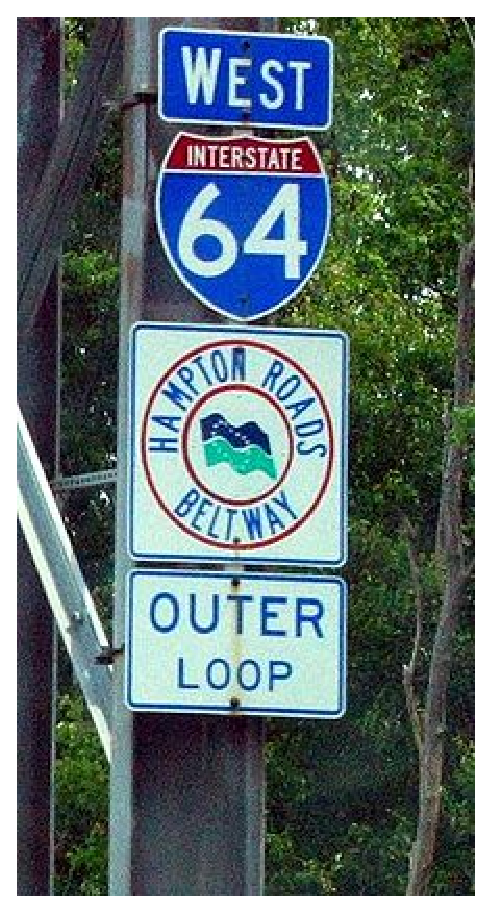
\includegraphics[height=9cm]{ring-11.eps}
  \end{center}
\end{frame}

\begin{frame}
  \frametitle{Над задачей работали}
  \begin{itemize}
    \item Идея задачи: Владимир Ульянцев
    \item Текст условия: Владимир Ульянцев
    \item Тесты, проверяющая программа и др.: Сергей Поромов
    \item Решения: Сергей Поромов, Сергей Мельников
    \item Текст разбора: Сергей Поромов
  \end{itemize}
\end{frame}

\begin{frame}
  \frametitle{Формулировка задачи}
  \begin{itemize}
    \item
      Дан монотонный многоугольник
    \item
      Необходимо построить вертикальную магистраль длиной ровно d
  \end{itemize}
\end{frame}

\begin{frame}
  \frametitle{Идея решения}
  \begin{itemize}
    \item Каждая вертикальная прямая пересекает многоугольник по не более, чем одному отрезку
    \item Интересные точки~--- всевозможные $x_i$
    \item На каждом отрезке между двумя интересными точками расстояние между верхней и нижней цепью изменяется линейно
          и потому либо не более одного подходящего места, либо бесконечно много
  \end{itemize}
\end{frame}

\begin{frame}
  \frametitle{Решение}
  \begin{itemize}
    \item Вариант 1 : отсортируем все $x_i$~--- решение за $O(n \log n)$
    \item Вариант 2 : найти самую левую и самую правую точку и бежать двумя указателями по верхней и нижней цепи~--- решение за $O(n)$
    \item Для каждого отрезка найти расстояние между верхней и нижней цепью~--- $d_l$ и $d_r$
    \item Если $d_l \le d < d_r$ или $d_r \le d < d_l$, то один вариант проведения магистрали
    \item Если $d_l = d = d_r$, то ответ~--- бесконечность
  \end{itemize}
\end{frame}

\begin{frame}
  \frametitle{Итого}
  \begin{itemize}
    \item Время работы есть $O(n \log n)$
    \item Вопросы?
  \end{itemize}
\end{frame}
